% 2009 年江苏卷第 18 题：圆 C1:(x+3)²+(y−1)²=4 与圆 C2:(x−4)²+(y−5)²=4。
% 来源 PDF：普通高考/2009/2009江苏.pdf
% SHA-256：64e417d45911d88d77c047a419dcc259e7c7dc779c79d20df2092755c96a4501
% 原页：2009江苏.pdf 第 1 页（A3 三栏）第 3 栏，书页码 531。
% 绘制依据：按原页坐标画两圆（半径均为 2）、坐标轴、圆心与点 A(4,0)。
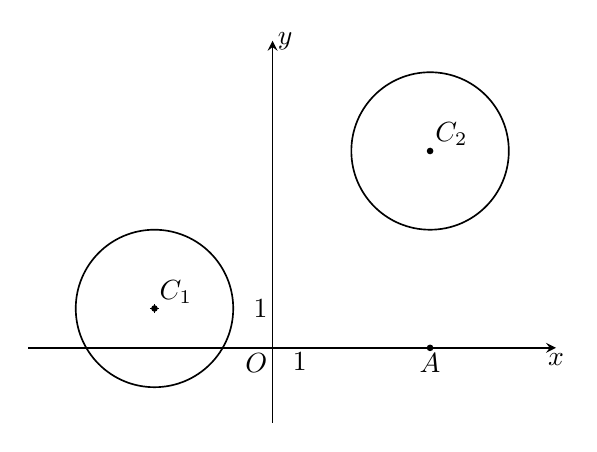
\begin{tikzpicture}[scale=0.5, semithick, every node/.style={inner sep=1.6pt}]
  \draw[->,>=stealth] (-6.2,0) -- (7.2,0) node[below] {$x$};
  \draw[->,>=stealth] (0,-1.9) -- (0,7.8) node[right] {$y$};

  \draw (-3,1) circle [radius=2];
  \draw (4,5) circle [radius=2];

  \fill (-3,1) circle (2.4pt);
  \fill (4,5) circle (2.4pt);
  \fill (4,0) circle (2.4pt);

  \draw (-3,1) ++(-0.12,0) -- ++(0.24,0);
  \draw (-3,1) ++(0,-0.12) -- ++(0,0.24);

  \node[above right] at (-3,1) {$C_1$};
  \node[above right] at (4,5) {$C_2$};
  \node[below] at (4,0) {$A$};
  \node[below left] at (0,0) {$O$};
  \node[below left] at (1,0) {$1$};
  \node[left] at (0,1) {$1$};
\end{tikzpicture}
